\chapter{Basic particle tracking pipeline}
\label{chap:basicpipeline}

Commonly, the particle tracking pipeline is split into the following sub tasks:
\begin{enumerate}
	\itemsep 0em
	\item \textbf{\locate* \textit{:}} considering each frame of each camera separately, find the pixel coordinates of all the bubbles in the image;
	\item \textbf{\link* \textit{:}} consider two consecutive time instants. For each bubble in the first frame, link it to where it moved in the next frame, to form \textbf{tracklets}. This step must take into account potential bubbles that appear or disappear;
	\item \textbf{\match* \textit{:}} consider corresponding frames of the different cameras. For each bubble in one camera, find which is, if any, the corresponding bubble in the other cameras. This information is then used to reconstruct the 3D position of the bubbles;
	\item \textbf{\visual* \textit{:}} display in a suitable way the reconstructed 3D scene on a 2D screen.
\end{enumerate}
In literature, some approaches follow the order 1-2-3-4 (blue in figure~\ref{fig:pipeline:order}), performing a camera-wise \link*.
Some other libraries chose to invert 2 and 3, obtaining a 1-3-2-4 order (orange in figure~\ref{fig:pipeline:order}).
This anticipates the 3D reconstruction before the \link*, thus performing a single \link* operation on 3D coordinate, obtaining 3D tracklets.

In the next paragraphs, each step will be analyzed separately.
For each step, I will compare all solutions found in literature among themselves, and with the ones developed by me, to find the overall best one.

\begin{figure}
	\centerline{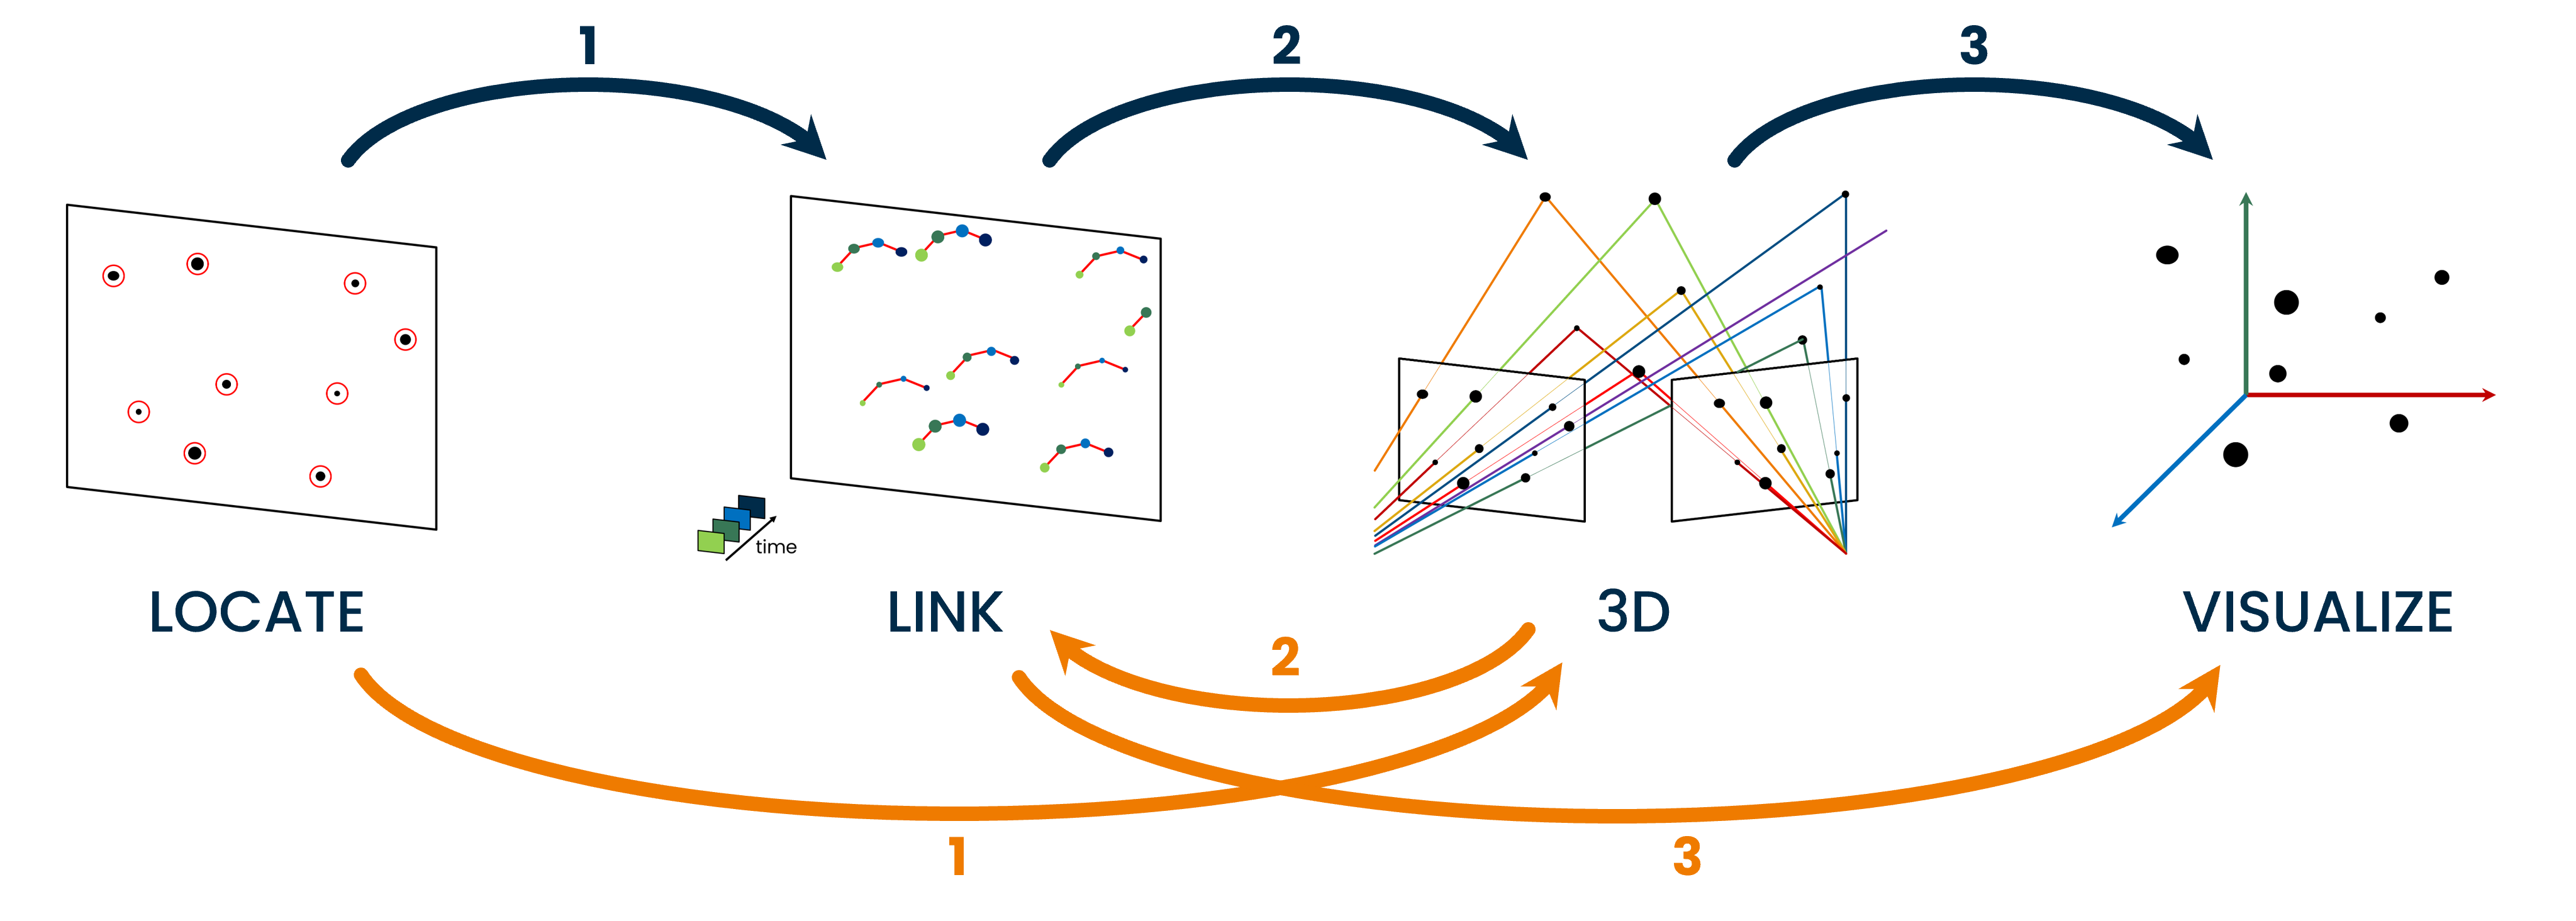
\includegraphics[width=\textwidth]{images/pipeline-orders.png}}
	\caption{\centering The two different orders in which the pipeline can be executed}
	\label{fig:pipeline:order}
\end{figure}
